\documentclass[a4paper,oneside,1,english1pt]{report}

\usepackage{graphicx}
\usepackage{indentfirst}
\usepackage{color}
\usepackage{setspace}
\usepackage[pdftex,pdfpagelabels,bookmarks,hyperindex,hyperfigures]{hyperref}
\usepackage{bookmark}
\usepackage[paper=a4paper,top=1in,bottom=1in,right=1in,left=1.5in]{geometry}

%\usepackage[printonlyused]{acronym}
\usepackage{acronym}



%%%%%%%%%%%%%%%%%%%%%%%%%%%%%%%%%%%%%%%%%%%%%%%%%%%%%%%%%%%%%%%%%%%%%%%%%%%%%%
% Terms and Acronyms


%%%%%%%%%%%%%%%%%%%%%%%%%%%%%%%%%%%%%%%%%%%%%%%%%%%%%%%%%%%%%%%%%%%%%%%%%%%%%%
%\usepackage{draftwatermark}
%\SetWatermarkText{
\includegraphics{logo/veritas.png}}
%\SetWatermarkColor[rgb]{1,0,0}

% to number subsubsection
\setcounter{secnumdepth}{3}
\setcounter{tocdepth}{3}

\begin{document}
%------------------------------------TITLE PAGE------------------------------------------------------------------------------------------------
\pagenumbering{roman}  %Roman page no.s for Front page 


\begin{titlepage}
	\newgeometry{margin=.5in}
	{
		\begin{center}
			
			%%%%% Uncomment to use veritas Logo
			%
\includegraphics[width=.2\linewidth]{logo/veritas.png}\\[.5cm]
			%\textbf{\LARGE Veritas Technologies LLC, Pune }\\
			
			
\includegraphics[width=.2\linewidth]{logo/walchand.jpg}\\[.5cm]
			\textbf{\LARGE Walchand College of Engineering, Sangli }\\
			\textbf {(An Autonomous Institute)}\\[.5cm]
			\textbf {\Large Department\\ of\\ Computer Science and Engineering}\\[1cm]
			{ \large \textbf{ A Project Report  } }\\
			on\\
			\textbf{\Large \color{blue}DevOps for Cloud Computing Environment }\\[1cm]
			%%%%%%%%%%%%%%%%%%%%%%
			\iffalse
			\textit \large{Submitted in partial fulfillment of the requirements for the award of degree of
				}\\[1cm]
			\textbf{BACHELOR OF TECHNOLOGY\\ IN \\COMPUTER SCIENCE AND ENGINEERING
				}\\[1cm]
			\fi
			
			\iffalse
			%%%%%%%%%%%%%%%%%%%%%%
			\large  {Members}\\[1cm]
			%	\end{center}
			{\setlength{\tabcolsep}{30pt}
				\renewcommand{\arraystretch}{1.5}
				\begin{tabular}{ll}
					\large{\textbf{Vaibhav Ananda Kumbhar} } & \large{\textbf{2012BCS057}} 
					%& \large\textbf{vkumbhar94@gmail.com}  
					
				\end{tabular}\\[1.5cm]
			}
			\fi
			\large  {Under the Guidance\\ of}\\[3cm]
			
			\begin{tabular}{c c}
							
				\begin{minipage}{.5\linewidth}
					\begin{center}
						\Large \textbf{ Prof. A. R. Surve  }\\
						\normalsize Guide\\
						Professor, Computer Science \& Engg Dept,\\
						WCE, Sangli\\
					\end{center}
				\end{minipage}
				&
				\begin{minipage}{.5\linewidth}
					\begin{center}
						\Large \textbf{ Mr. Prasanna Kulkarni  }\\
						\normalsize Co-Guide\\
						Senior Manager,\\
						Veritas Technologies LLC, Pune
					\end{center}
					
				\end{minipage}\\
				
			\end{tabular}\\[1cm]
			Submitted\\
			by\\[2cm]
			{\setlength{\tabcolsep}{30pt}
				\renewcommand{\arraystretch}{1.5}
				\iffalse
				\begin{tabular}{ll}
					\large{\textbf{Vaibhav Ananda Kumbhar} } & \large{\textbf{2012BCS057}} 
					%& \large\textbf{vkumbhar94@gmail.com}  
				\end{tabular}\\[1.5cm]
				\fi
				\large{\textbf{Vaibhav Ananda Kumbhar}}\\[.5cm]
				 \large{\textbf{2012BCS057}}
			}
			%	\begin{center}
			\vfill
			\large \textbf{2015-2016 }\\[.4cm]
			
		\end{center}
	}
\end{titlepage}



\newpage
%\begin{titlepage}
%\begin{stretchbox}
{	
	\linespread{2}
	
	\begin{center}
		
\includegraphics[width=.2\linewidth]{logo/walchand.jpg}\\[.5cm]
		\textbf{\Large Walchand College of Engineering, Sangli }\\
		\textbf {(An Autonomous Institute)}\\[.5cm]
		\textbf {\LARGE Department of Computer Science and Engineering}\\[1cm]
		\huge \textbf{\textcolor{blue}{\underline{CERTIFICATE}}}\\[1cm]
	\end{center}
	\linespread{1.6}
	\par \large This is to certify that the B.Tech. Project entitled \textbf{DevOps for Cloud Computing Environment} is a bonafide work carried out by \textbf{ Mr. Vaibhav Ananda Kumbhar} in partial fulfillment of the completion of B. Tech. project during the year 2015-2016. The project report has been approved as it satisfies the academic requirement with respect to the project work.\\[5cm]
	%\vfill
	\begin{tabular}{c c c}
		
		\begin{minipage}{.30\linewidth}
			\begin{center}
				\normalsize \textbf{ Prof. A. R. Surve  }\\
				\normalsize Guide\\
				Professor, CSE Dept,\\
				WCE, Sangli\\
			\end{center}
		\end{minipage}
		&
		\begin{minipage}{.35\linewidth}
			\begin{center}
				\normalsize \textbf{ Mr. Prasanna Kulkarni  }\\
				\normalsize Co-Guide\\
				Senior Manager,
				Veritas Technologies LLC, Pune
			\end{center}
			
		\end{minipage}
		&
		
		\begin{minipage}{.35\linewidth}
			\begin{center}
				\normalsize \textbf{ Prof. Dr. B. F. Momin  }\\
				\normalsize HOD\\
				CSE Dept,\\
				WCE, Sangli\\
			\end{center}
		\end{minipage}
	\end{tabular}
	%\end{stretchbox}
	
	%\end{titlepage}
}


%----------------------------------Contents--------------------------



\restoregeometry
\doublespacing

\iffalse
\begin{abstract}
	AJKAHKDJADHK
\end{abstract}
\fi

\newpage

\begin{center}
	\textbf{\Huge Acknowledgement}\\[2cm]
\end{center}
	\par I wish to take this opportunity to express my sincere gratitude to all the people who have extended their cooperation in various ways during my project work. It's my pleasure to acknowledge all those individuals.\\
	
	I wish to express my sincere gratitude to Mr. Prasanna Kulkarni, Co-guide,  Senior manager, and Mr. Aatish Arora, Senior Manager, for providing me an opportunity to do my internship and project work in "VERITAS TECHNOLOGIES, LLC".
	With their guidance, cooperation and encouragement, I learnt various new things during our project tenure.\\
	
	I would like to thank my project guide Prof. A. R. Surve sir, Computer Science and engineering Department for his guidance and help throughout the development of this project work by providing me with required information.\\
		
	I would like to thank all my team members in VERITAS who helped me in every aspect to complete this project successfully.\\
	

	I specially thank Dr. B. F. Momin Head, Computer Science and Engineering Department for his continuous encouragement and valuable guidance in bringing shape to this dissertation.\\
	
	I specially thank Dr. G.V. Parishwad, Director, of Walchand College of Engineering, Sangli	for his encouragement and support.
	

	
\newpage

\begin{center}
	\textbf{\Huge Declaration}\\[2cm]
\end{center}
 \par I hereby declare that the project work entitled
 \textbf{"DevOps for Cloud Computing Environment"}
 submitted to the Walchand College of Engineering, Sangli is a record of an original work done by me under the guidance of \textbf{Prof. A. R. Surve, Computer Science \& Engineering} and  \textbf{Mr. Prasanna Kulkarni, Senior Manager, VERITAS Technologies LLC.,Pune} and this project work is submitted in the partial fulfillment of the requirements for the award of the degree of Bachelor of Technology in Computer Science \& Engineering.\\[3cm]
 

\begin{tabular}{c c c}
	
\begin{minipage}{.3\linewidth}
\begin{flushleft}
	Date:\\
	Place: 
\end{flushleft}		
\end{minipage}
&
\begin{minipage}{.3\linewidth}
	.
\end{minipage}
&
\begin{minipage}{.4\linewidth}
\begin{flushleft}
	Vaibhav A. Kumbhar\\
	2012BCS057,\\
	B.Tech. C. S. E.
\end{flushleft}	
\end{minipage}
\end{tabular}

\newpage

\begin{center}
	\textbf{\Huge Abstract}\\[2cm]
\end{center}
\par Today the IT development is growing very fast. Customer needs updates of product more frequently. The code quality should be good so that improvement and bug fixing in the product will be more easily and quickly. 
\par The purpose of \textbf{DevOps for Cloud Computing Environment} is to do software development fast and seamlessly by minimizing the gap between developers teams and other IT operations teams. \ac{VRP} will be able to release products more frequently.
\par In this project's context, we focuses on the source code analysis. The source code should be well tested so that it will eventually improves code quality.






\pdfbookmark{\contentsname}{Contents}
\addtocontents{toc}{~\hfill\textbf{Page}\par}
\tableofcontents

%\pdfbookmark{List of Figures}{List of Figures}
\listoffigures
\addcontentsline{toc}{chapter}{List of Figures}

%\listoftables
\newpage





\section*{\Huge List of Acronyms}
\addcontentsline{toc}{chapter}{List of Acronyms}
\begin{acronym}[AWGN]
	\acro{CI/CD}{Continuous Integration and Continuous Delivery}
	\acro{CI}{Continuous Integration}
	\acro{CD}{Continuous Delivery}
	\acro{VRP}{Veritas Resiliency Platform}
	\acro{POM}{Project Object Model}
	\acro{JaCoCo}{Java Code Coverage}
	\acro{DC}{Data Center}
	\acro{VCS}{Version Control System}
	\acro{SCM}{Software Configuration Management}
	\acro{LOC}{Lines of Code}
	\acro{KLOC}{Thousands lines of code}
	\acro{IDE}{Integrated Development Environment}
	\acro{VSA}{Virtual Service Appliance}
\end{acronym}

\clearpage
\pagenumbering{arabic} %Arabic for chapters
\chapter{\uppercase{Introduction}}	
\section{Introduction to DevOps}
	\begin{figure}
		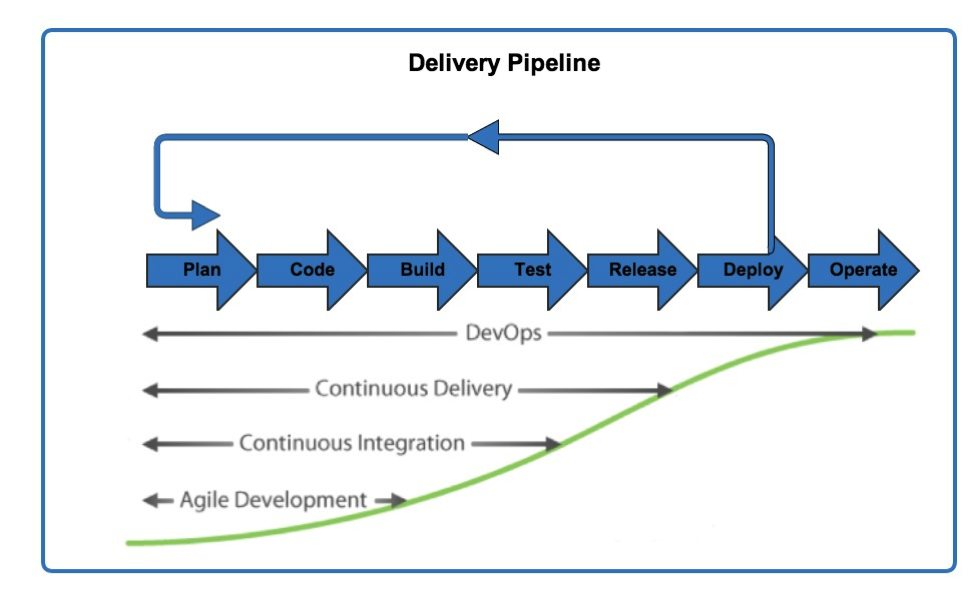
\includegraphics[width=.8\linewidth]{diagrams/all.png}
		\caption{Delivery Pipeline \cite{DeliveryPipeline}}
		\label{fig:delivery_pipeline}
	\end{figure}

	What is DevOps? DevOps is a culture that company can use it to develop big projects seamlessly to achieve fast development and delivery of products to customer by collaborating developers and operations team together.

	\par A few decades back, almost all systems were standalone. But nowadays, everybody wants access to application from anywhere at any time. That's why web applications became more popular. 
	Instead of dedicated servers, in today's era, cloud computing is becoming more popular and it is where shared resources, data and information are provided to computers and other                                devices on-demand.
	
	
	\par As cloud computing environments are distributed and virtualization needs to be extensively used, it is more complex to develop a cloud based solution.
	We need to implement DevOps for cloud computing environment so that the development of cloud based solutions will become easier. We can help operations and development engineers participating together in the entire service lifecycle, from design through the development process to production support. 
	\par Scope of DevOps includes phases from planning to the actual deployment of product as shown in figure \ref{fig:delivery_pipeline}. DevOps tries to cover the delivery flow of product from phase planning to deployment. DevOps ensures that the Continuous Integration and Continuous Delivery has been achieved.
\section{Introduction to Cloud Computing Environment}
	Cloud computing is single point of interaction to user with distributed hardware resources. Virtualization technologies are used by cloud computing environment.   Openstack is one open source  software to enable cloud technology.
	\par Main two types of cloud are as following: Public cloud, private cloud. Private clouds are installed by their own organization. Public clouds, like AWS, etc., can be used on the basis of resource usage and cloud service provider/cloud vendor charge for it.
	
\section{Introduction to \ac{VRP}}
	Veritas Resiliency Platform (\ac{VRP}) provides resiliency to virtual machines in the data centers by using cloud data center as secondary/recovery data center. The various virtualization technologies like Hyper-V and VMware supported by \ac{VRP} for resiliency.
	The cloud data centers used as secondary data center for recovery in case of disaster. Openstack cloud technology supported for secondary data centers.\\
	VRP handles these various technologies, so to integrate them altogether and to develop product fast and seamlessly, to implement DevOps was necessary.
\section{Continuous Integration and Continuous Delivery}
	\begin{figure}
		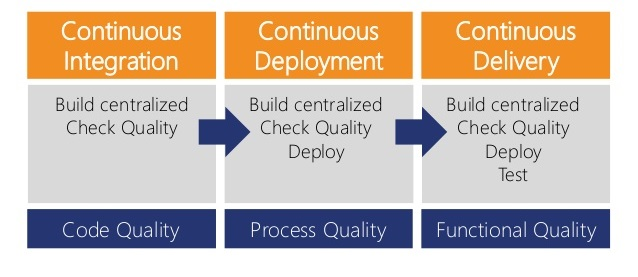
\includegraphics[width=.8\linewidth]{diagrams/CICD.jpg}
		\caption{Continuous Integration vs Continuous Delivery vs Continuous Deployment \cite{CI/CD/CD}}
		\label{fig:CI-CD}
	\end{figure}
	\par
	\ac{CI} is a approach of integrating all working copies of developers on central shared mainline without causing failures to each others code. Developers can be able see how their change in existing or new code will behave into the actual product.
	\par
	\ac{CD} is a approach in which teams produce software in short cycles. Each cycle ensures that we can release high quality software fast through build, test and deployment automation.
	The benefits we can get from this is that it reduces the cost, time, and risk of delivering changes. We will be able to do incremental updates easily and more frequently. Agile methodology is best suited to achieve continuous delivery(\ac{CD}). Development life cycle is divided into number of short cycles known as sprints. At the end of each sprint every story has to be completed so that after every sprint release team can be able to release product.
	\par "Continuous Integration" ensures code quality by checking compatibility with another's code. "Continuous Delivery" ensures the functional quality whether it is can be deployable or not. It checks only  proper functionality, It does not deploys product anymore. "Continuous Deployment" ensures the process quality by test, automation acceptance testing and then product deploys automatically.
	Relevance between these three terms is shown in figure \ref{fig:CI-CD}
\chapter{\uppercase{Technical Specifications}}

	\section{Project Management}
		\par Maven is software project management tool. The projects distributed  among various team working on various technologies can be dependent on each other. Maven is best suited to develop products in multi module environment projects.
		Maven is based on declarative model. It defines  \ac{POM} in pom.xml file\\
		\subsection{Maven Operations}
		\par  Maven can do following operations:
		\begin{enumerate}
			\item Builds: Makes build process easy. It takes source code, compiles it and packages them into executables.
			\item Reporting: It generates reports as well which includes build log, used third party plugins in project.
			\item Documentation: Keeps project description, summary.
			\item Dependencies: Keeps track of third party plugin dependencies. And it keeps track of dependencies between child modules in same project.
			\item \ac{SCM}s: Maven can push code automatically  to version control system if the build succeed and it also includes the recent changes done with respect to previous build and who did that changes.
			\item Releases: Maven handles the release management by using project versions and update to next version. Maven can rollback to previous version.
			\item Distribution: Maven puts repositories on server. Anyone can download latest build/executable from there.
			\item Mailing list: Maven puts mailing list on site to subscribe/unsubscribe. Email will be broadcast to all members.
		\end{enumerate}
	\subsection{Maven Lifecycle}
	\par Maven works around build cycle. Following are the maven phases of lifecycle:
		\subsubsection{Clean Lifecycle}
		\par Clean lifecycle removes the files and folders created by previous build. Phases in clean lifecycle are as following:
				\begin{enumerate}
					\item pre-clean: 	execute processes needed prior to the actual project cleaning
					\item clean: 	remove all files generated by the previous build
					\item post-clean: 	execute processes needed to finalize the project cleaning
				\end{enumerate}
			\subsubsection{Build Lifecycle}
			\par Build lifecycle actual produces software deliverables like .jar or .exe files. Phases in build lifecycle are as following:
				\begin{enumerate}
					\item validate:	validate the project is correct and all necessary information is available.
					\item initialize: 	initialize build state, e.g. set properties or create directories.
					\item generate-sources: 	generate any source code for inclusion in compilation.
					\item process-sources: 	process the source code, for example to filter any values.
					\item generate-resources: 	generate resources for inclusion in the package. It copies resources from the resources directory into the output directory to include it into the installable file like jar.
					\item process-resources: 	copy and process the resources into the destination directory, ready for packaging.
					\item compile: 	compile the source code of the project.
					\item process-classes: 	post-process the generated files from compilation, for example to do bytecode enhancement on Java classes.
					\item generate-test-sources: 	generate any test source code for inclusion in compilation.
					\item process-test-sources: 	process the test source code, for example to filter any values.
					\item generate-test-resources: 	create resources for testing. It generates the resources required while testing in test  resources directory.
					\item process-test-resources: 	copy and process the resources into the test destination directory.
					\item test-compile: 	compile the test source code into the test destination directory
					\item process-test-classes: 	post-process the generated files from test compilation, for example to do bytecode enhancement on Java classes. For Maven 2.0.5 and above.
					\item test: 	run tests using a suitable unit testing framework. These tests should not require the code be packaged or deployed.
					\item prepare-package: 	perform any operations necessary to prepare a package before the actual packaging. This often results in an unpacked, processed version of the package. (Maven 2.1 and above)
					\item package: 	take the compiled code and package it in its distributable format, such as a JAR.
					\item pre-integration-test: 	perform actions required before integration tests are executed. This may involve things such as setting up the required environment.
					\item integration-test: 	process and deploy the package if necessary into an environment where integration tests can be run.
					\item post-integration-test: 	perform actions required after integration tests have been executed. This may including cleaning up the environment.
					\item verify: 	run any checks to verify the package is valid and meets quality criteria.
					\item install: 	install the package into the local repository, for use as a dependency in other projects locally.
					\item deploy: 	done in an integration or release environment, copies the final package to the remote repository for sharing with other developers and projects.
					
					
				\end{enumerate}
			\subsubsection{Site Lifecycle}
			\par Site lifecycle generates site for the project regarding build information. Site includes information about the third party used plugins, artifacts of current build version, etc. Phases in site lifecycle are as following:
				\begin{enumerate}
					\item pre-site: 	execute processes needed prior to the actual project site generation
					\item site: 	generate the project's site documentation
					\item post-site: 	execute processes needed to finalize the site generation, and to prepare for site deployment
					\item site-deploy: deploy the generated site documentation to the specified web server
				\end{enumerate}
	\subsection{Maven Profile}
	\label{maven:profile}
		\par In Maven, we can define specific configuration in profile. When that profile activates then the executions defined in that profile runs. We can define multiple profiles for different goals. Profile has multiple goals which are associated with any phase of lifecycle.\\
		
		For ex.: To clean the directory other than default output directories, needs to be delete in clean phase of clean lifecycle. To delete that directory, we could specify goal.
		We can activate one or more profiles at a time.
	\section{Continuous Integration}
		\par Jenkins is a automation server. Professionals uses it to build software products. Once  Jenkins configuration is ready, then it downloads source code from central repositories like stash, git hub, bit bucket, etc. and builds the software.
		\par Jenkins can schedule periodic build. Several build are fired in one day so that the developers can test their code latest build.
	\section{Continuous Delivery}
		Agile methodology is best to achieve continuous delivery. JIRA is project development and issue tracking tool. At the beginning of every sprint, a story has been decided first then actual development starts.  Once story  decides then it is divided into small tasks and for every task incident on JIRA created. At the end of sprint all JIRA incidents should be resolved and completed without any defect.
	\section{Code Coverage}
		What is Code Coverage? The Code Coverage means to check whether the code written by developer is well tested or not. JaCoCo is java code coverage tool which instruments java code and determines coverage matrices. JaCoCo is best because it does the instrumentation on-the-fly while unit testing, so there is no need to do offline instrumentation. On-the-fly instrumentation reduces overall time to build and analysis.
		\cite{jacoco-metrics}
		\subsection{Code Coverage Counters}
		\par Units to measure code coverage by  various techniques depending on different behaviors of code elements.
		\begin{enumerate}
			\item {\textbf{Instruction Coverage}:
				Typically it is related to the java byte code instructions. This counter indicates percentage of instructions covered by unit testing.
				}
			\item {\textbf{Branch Coverage}:
				 Includes the IF-ELSE, SWITCH, etc code element which lead to branching.
				 Source Code Highlighters:
				 
				 \begin{itemize}
				 	\item Red diamond: No coverage.
				 	\item Yellow diamond: Partial coverage. Some branches covered.
				 	\item Green diamond: Full coverage.
				 \end{itemize}
				}
			\item {\textbf{Line Coverage}:
				This column depicts how many lines in source code has been covered by  unit testing. Line counter unit is \ac{LOC}/\ac{KLOC}.
				}
			\item {\textbf{Method Coverage}:
					Coverage percentage of method covered in unit testing. If any branch inside the method is uncovered then the method will be marked as uncovered.
				}
			\item {\textbf{Class Coverage}:
				The class has been instantiated or not determines class coverage. If the class is not instantiated in unit testing, then class will be marked as uncovered.
				}
		\end{enumerate}
	
		\subsection{Cyclomatic Complexity}
		Number of linearly independent paths in source code. It determines number of test cases required to cover all source code.
		for ex:
		\begin{itemize}
			\item \textbf{If-else}: Only one section will execute either if block or else block thats why complexity would be 1.
			\item Only \textbf{IF} condition no else section: When \textit{IF} condition becomes true that would be one path and if the \textit{IF} condition false that would be another path so complexity would be 2.
			\item If \textbf{IF} condition with two condition then complexity would be 2.
		\end{itemize}
\chapter{\uppercase{System Analysis}}
	\section{Overview}
		\par  All developers, QA team and  other IT operations teams analyzes unit test report and makes decision to accept code for further testing. All developers will be able to analyze their own code locally.
	\section{Proposed System}
	
		\par DevOps is partially implemented for \ac{VRP}. One Jenkins project to do coverage analysis and publishes results to all teams. 
		\par Unit testing should be done in parallel so that it will optimize execution time. Along with unit tests, system collects the coverage statistics. After complete execution the system will publish reports and sends report link to all people who are working on \ac{VRP}.
	\section{Hardware Requirements}
		\begin{itemize}
			\item x86 processor Desktop/Laptop.
		\end{itemize}
	\section{Software Requirements}
		\begin{itemize}
			\item Maven
			\item Eclipse
			\item JaCoCo
			\item Jenkins
		\end{itemize}
	
\chapter{\uppercase{System Design}}

\section{Architecture Diagram}

\begin{figure}[h]
	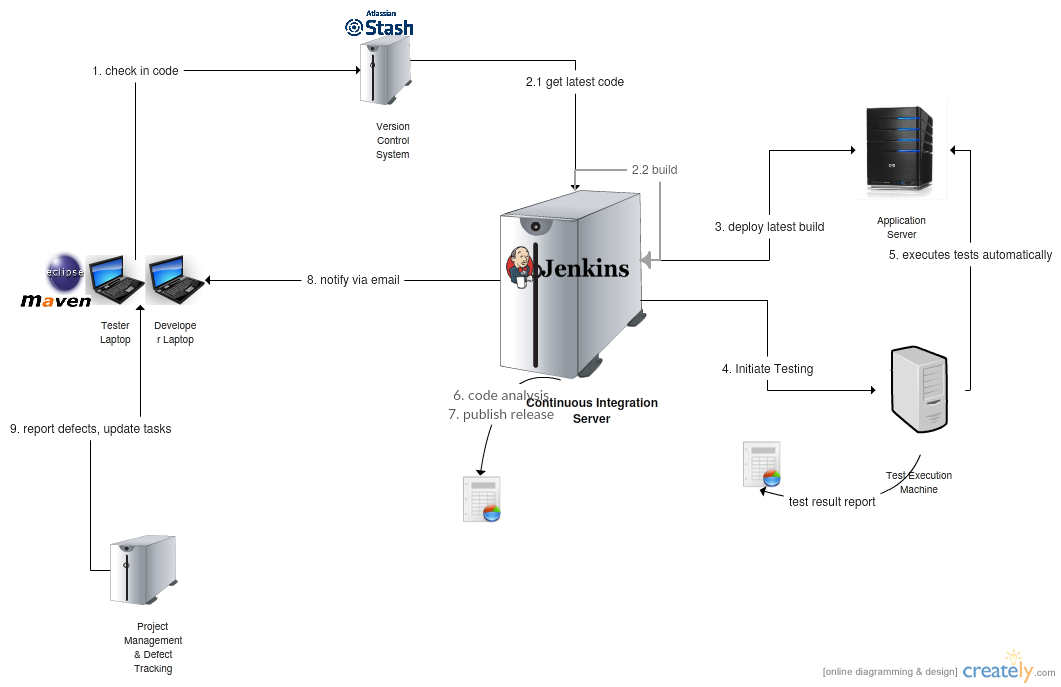
\includegraphics[width=\linewidth]{diagrams/Arch diagram.png}
	\caption{Architecture Diagram}
	%  for Continuous Integration
	\label{fig:arch_dia}
\end{figure}
DevOps system comprises of the components shown in the figure \ref{fig:arch_dia}.
Jenkins \ac{CI} server plays vital role in DevOps. Jenkins \ac{CI} server is central place to all people working in project.\\

\subsection{Architecture Explanation}
	Data flow and sequence of activities are shown in the figure \ref{fig:arch_dia}. Some more information of activities included in architecture is  as following:
\begin{enumerate}
	\item \textbf{Check in code}:
	Developer writes code and merges it with repository on \ac{VCS}. Similarly, Tester writes test cases and merges it with repository on \ac{VCS}.
	
	\item \textbf{Build}: Jenkins \ac{CI} server gets latest updated code from repository and builds the product.
	\begin{enumerate}
		\item Get latest code: Copies source code repository from \ac{VCS} to the Jenkins workspace.
		\item Build: Builds the product from copied source code and generates all executables.
	\end{enumerate}
	
	\item \textbf{Deploy latest build}: \ac{CI} server deploys latest build on application server and configures it. \ac{CI} server starts  software product service on application server.
	
	\item \textbf{Initiate testing}: Once application is ready, then \ac{CI} server initiates testing. 
	
	\item \textbf{Execute tests}: Test execution machine  starts tests on app;ication server one by one automatically and collects log for test cases both passed and failed.
	
	\item \textbf{Code analysis}: Code analysis starts on the source code which were used to build product.
	
	
	\item \textbf{Publish release}:
	Once the source code analysis and the testing done application server done then publishes release reports. Reports includes the test report and code analysis report. Once reports analyzed by release team then product will be ready for release.
	
	\item \textbf{Notify via email}:
		If any code broken in build phase then \ac{CI} server notifies the respective developer or tester with the failure log.
	\item \textbf{Report defects and update tasks}:
		Once product has been released then the real time defects arises from the customer. Customer gives suggestions to add new feature. Accordingly the new tasks created and given to the developer for implementation.
\end{enumerate}


\section{UML Diagrams}
\subsection{Use Case Diagram}

\iffalse
\begin{figure}[h]
	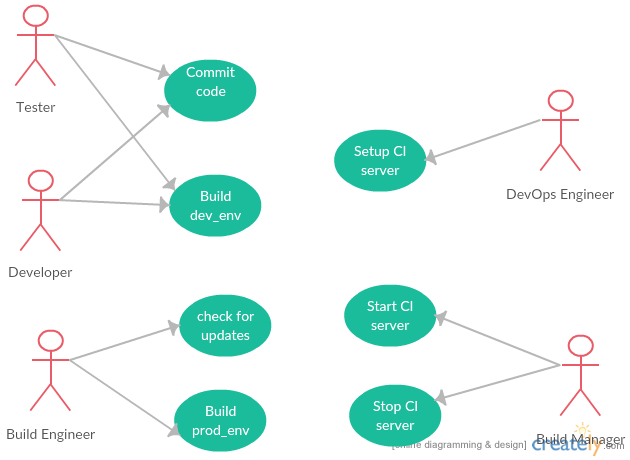
\includegraphics[width=\linewidth]{diagrams/CI_Use_Case1.png}
	\caption{Use Case Diagram}
	%  for Continuous Integration
	\label{fig:use_case_dia}
\end{figure}
\fi

Use cases included in DevOps are as following.
\iffalse
Build dev\_env use case called by developer. He can be able to see coverage analysis on his machine.
\fi

\subsubsection{DevOps Use Case}
\begin{figure}[h]
	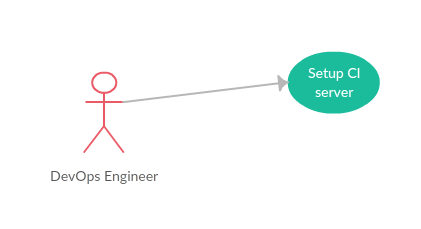
\includegraphics[width=\linewidth]{diagrams/DevOpsUseCase.png}
	\caption{DevOps Use Case Diagram}
	%  for Continuous Integration
	\label{fig:devops_use_case_dia}
\end{figure}
DevOps Use Case view shown in figure \ref{fig:devops_use_case_dia}. DevOps engineer is one actor who has very important role in the product. He is the one person who handles all product development and delivery process. DevOps engineer has to setup the DevOps system. \ac{CI} server is central component in DevOps system. DevOps engineer is caller of  \textit{setup \ac{CI} server} use case.


\begin{figure}[h]
	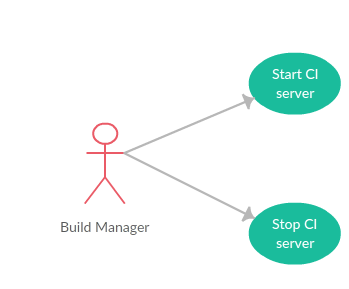
\includegraphics[width=\linewidth]{diagrams/BuildManagementUseCase.png}
	\caption{Build Management Use Case Diagram}
	%  for Continuous Integration
	\label{fig:buildmanagement_use_case_dia}
\end{figure}
\subsubsection{Build Management Use Case}
Build Management Use Case view shown in figure \ref{fig:buildmanagement_use_case_dia}. Build manager is on top of all who has all rights. If he wants to stop DevOps system he will call \textit{stop \ac{CI} server}. Similarly, he wants to start DevOps system he calls \textit{start \ac{CI} server}.

\begin{figure}[h]
	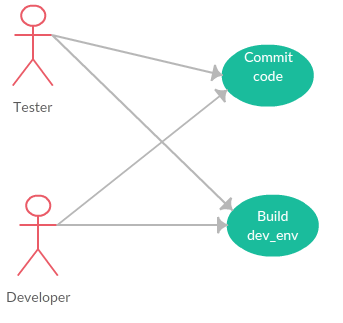
\includegraphics[width=\linewidth]{diagrams/DevelopmentUseCase.png}
	\caption{Development Use Case Diagram}
	%  for Continuous Integration
	\label{fig:development_use_case_dia}
\end{figure}
\subsubsection{Development Use Case}
	Development Use Case view shown in figure \ref{fig:development_use_case_dia}. This includes two use cases one is commit code and another is build product under development environment. Developer and Tester are two actors calls these use cases.
	Actors playing role in this:
	\begin{enumerate}
		\item Developer: Developer wants to build product with his changes. He calls \textit{build } under dev environment. Once he is done with correct changes then he \textit{commits code} and pushes it central repository.
		\item Tester: Tester writes test cases and builds product with his test cases. If his test cases are completed  then he adds his test cases to central repository by calling commit code.
	\end{enumerate}

\begin{figure}[h]
	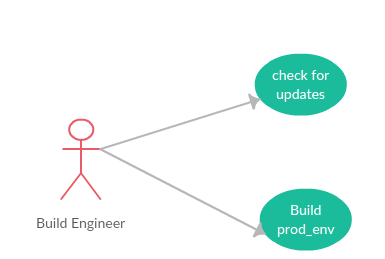
\includegraphics[width=\linewidth]{diagrams/BuildUseCase.png}
	\caption{Build Use Case Diagram}
	%  for Continuous Integration
	\label{fig:build_use_case_dia}
\end{figure}
\subsubsection{Build Use Case}
	Build Use Case view shown in figure \ref{fig:build_use_case_dia}. Build engineer is one actor plays role in build use case. Build engineer checks the updations in source code repository periodically by calling \textit{check for updates}. If new changes found in latest source code, he fires \textit{build}.
	\textit{Build prod\_env} use case called by build engineer,  \ac{CI} server via scheduled build or by any user via parameterized build.
	
\subsection{Class Diagram}
\begin{figure}[h]
	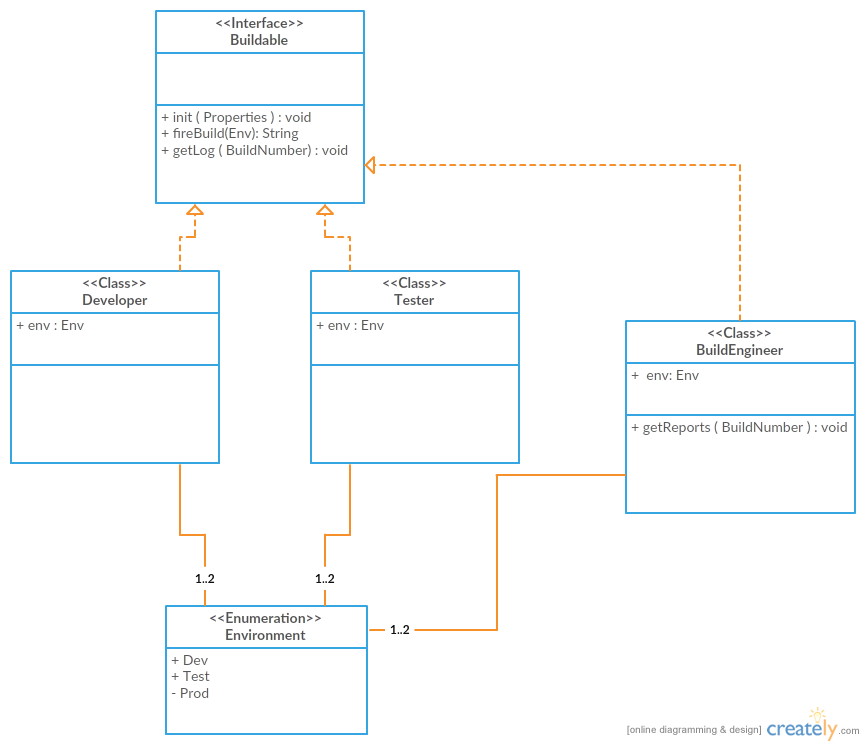
\includegraphics[width=\linewidth]{diagrams/ClassDiagram2.png}
	\caption{Class Diagram}
	%  for Continuous Delivery
	\label{fig:class_diagram}
\end{figure}
	Class diagram shown in figure \ref{fig:class_diagram}.
	Details of classes in class diagram.
		
	\subsubsection{Environment}
	Environment enumeration to set environment according to type of environment. Types of environment are Development, Test and production.
	
	\subsubsection{Buildable}
	This is interface defines two behaviors for classes. \textit{init} behavior initializes environment. \textit{fireBuild} starts build of product. Implementer of this interface has to write this behavior.
		
	\subsubsection{Developer}
	Developer can \textit{fire build} and \textit{get log} of that build.
		
	\subsubsection{Tester}
	Tester can fire build with test environment enabled and get log of test case execution.
		
	\subsubsection{Build Engineer}
	Build engineer can fire build and get log of that build. He also can get the high level reports of that build which includes the information of successful build.
\subsection{Sequence Diagram}
\begin{figure}[h]
	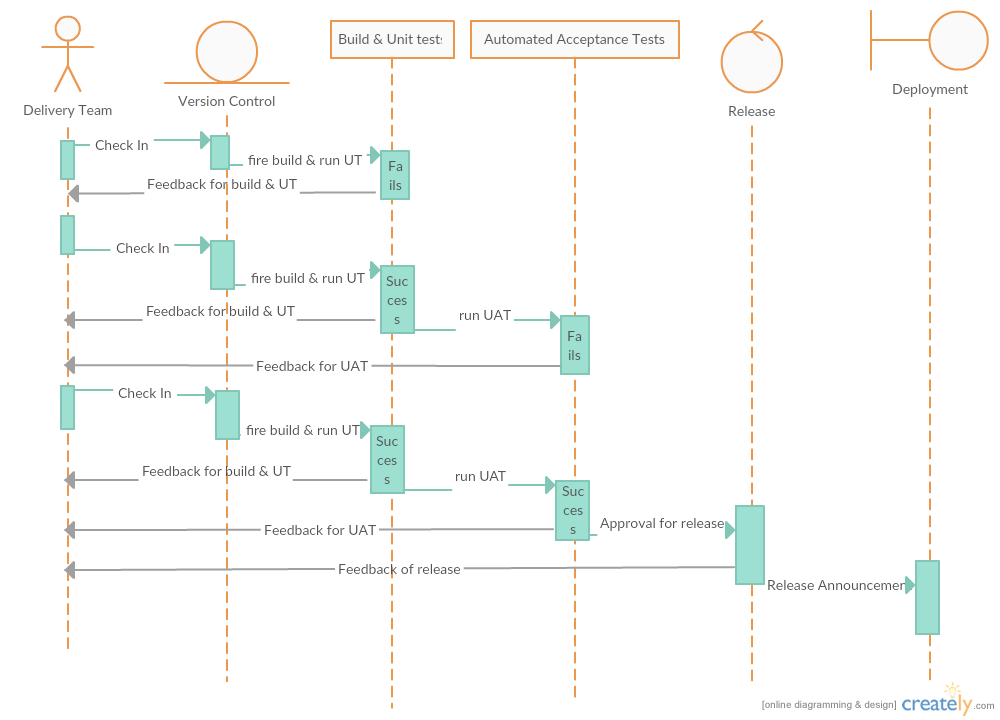
\includegraphics[width=\linewidth]{diagrams/SequenceDiatransp2.png}
	\caption{Sequence Diagram}
	%  for Continuous Delivery
	\label{fig:seq_dia}
\end{figure}
 Sequence of operations in DevOps as shown in figure \ref{fig:seq_dia}.
	
	
	Lifelines in the sequence diagram as following:

		\subsubsection{Delivery Team}
			Delivery team is actor  who is triggering all the sequence of operations. 	
		\subsubsection{\ac{VCS}}
		\ac{VCS} is a Entity lifeline where source code of product is available.
		
		\subsubsection{Build \& unit tests}
		Lifeline from which sequence can be stopped if any failure in the build and unit testing. If builds successfully then triggers next sequence.
	
		\subsubsection{Automated acceptance tests}
		Controller lifeline, managed by test execution machine, tests the system by running automated test cases.
		
		\subsubsection{Release}
		Release is controller lifeline where product release can be declined or approved.
		
		\subsubsection{Deployment}
		Deployment is boundary lifeline. Once this lifeline boundary reached the product will ready to release.\\
\chapter{\uppercase{Implementation}}
	\section{Development Environment}
		Eclipse is open source IDE used by almost all developers. For eclipse environment defined one build configuration by enabling JaCoCo instrumentation. Integration of JaCoCo with eclipse done by writing one maven profile \ref{maven:profile}. Within profile, executions defined for prepare-agent (which does the instrumentation) and report(generates report).
	\section{Production Environment}
		\par Jenkins is used to build \ac{VRP}. One Jenkins projects is created for code coverage analysis. Project publishes coverage result to all teams of \ac{VRP} by email. Thresholds has been set to accept code for further testing.
		
\chapter{\uppercase{System Testing}}
	\section[Developer Team]{Developer Team}
		\par Developer team uses eclipse as development environment to build product and test their written code. Developer has to fire build with unit test by enabling JaCoCo instrumentation.
		Once build succeed without error and test failure, code coverage report will be available in report output  directory. Developer has to ensure that the collecting coverage statistics and report is correct.
	\section[Build Team]{Build Team}
		\par Build team uses Jenkins \ac{CI} server to collect and view coverage statistics. Build team has to ensure that all builds are going in proper without harming other project or parallel build.
	\section[QA Team]{QA Team}
		\par QA team ensures that the functional testing code coverage is up to the mark to consider it for further testing.
\chapter{\uppercase{Screenshots and Results}}
	\section{Screenshots}
		\begin{figure}[h]
			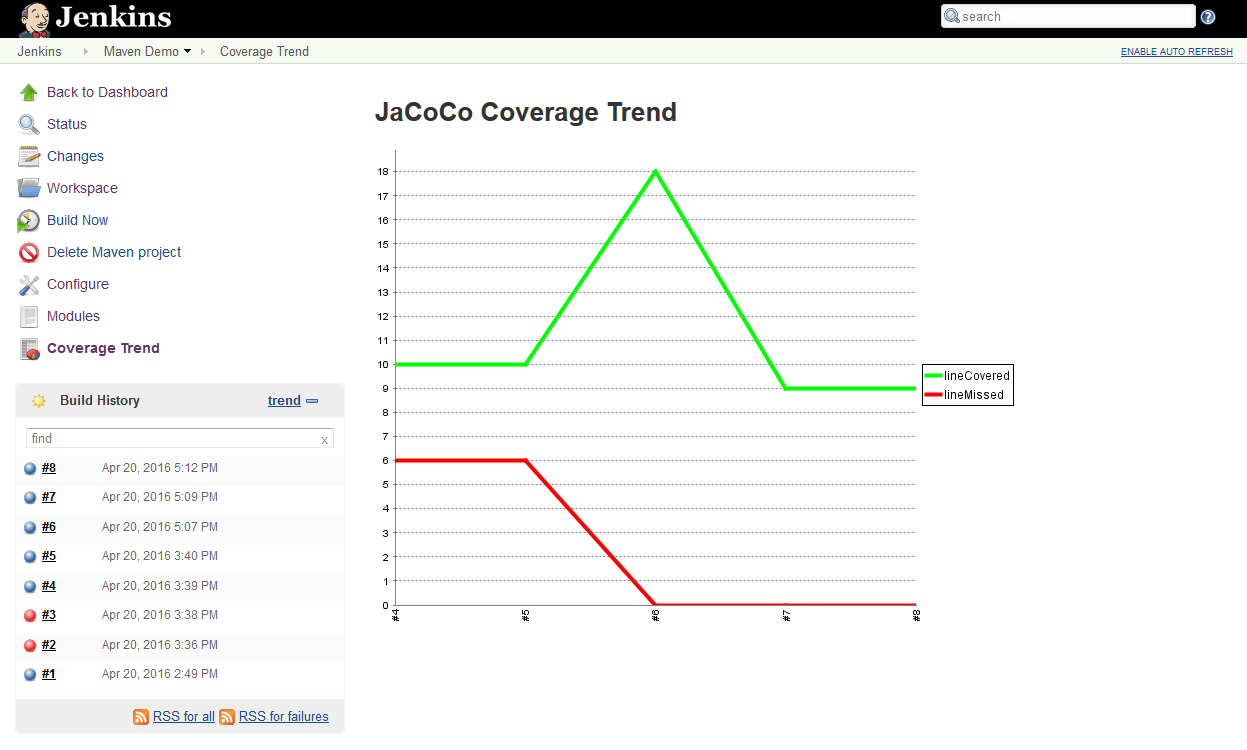
\includegraphics[width=\linewidth]{screenshots/CoverageTrend.png}
			\caption{Code Coverage Trend}
			
		\end{figure}
		
		\begin{figure}[h]
		\includegraphics[width=\linewidth]{screenshots/CoverageReport.png}
			\caption{Code Coverage Report}
			
		\end{figure}
		
		
		\begin{figure}[h]
			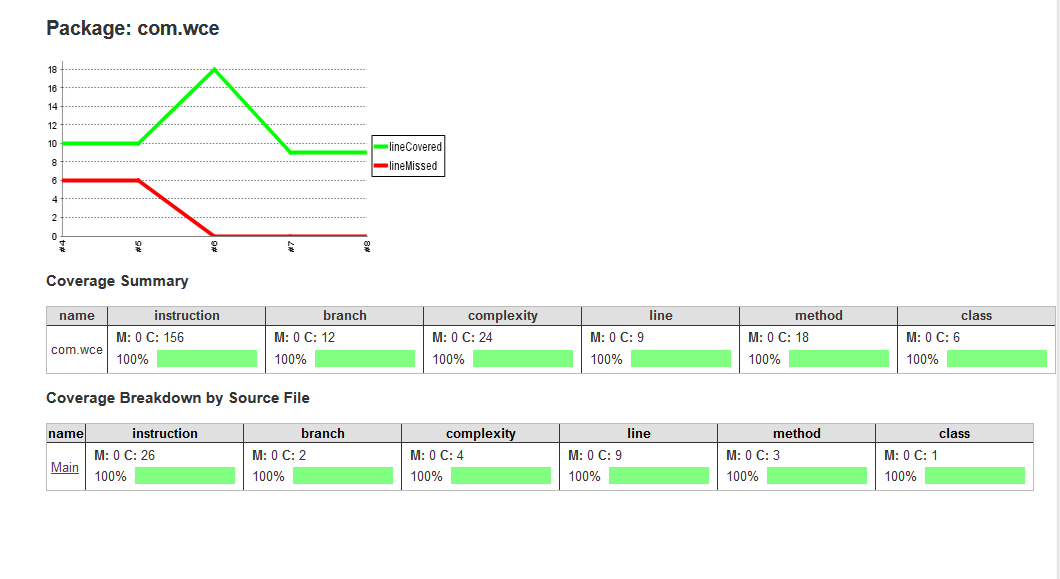
\includegraphics[width=\linewidth]{screenshots/PackageCoverage.png}
			\caption{Package Coverage}
			
		\end{figure}
		
		
		\begin{figure}[h]
			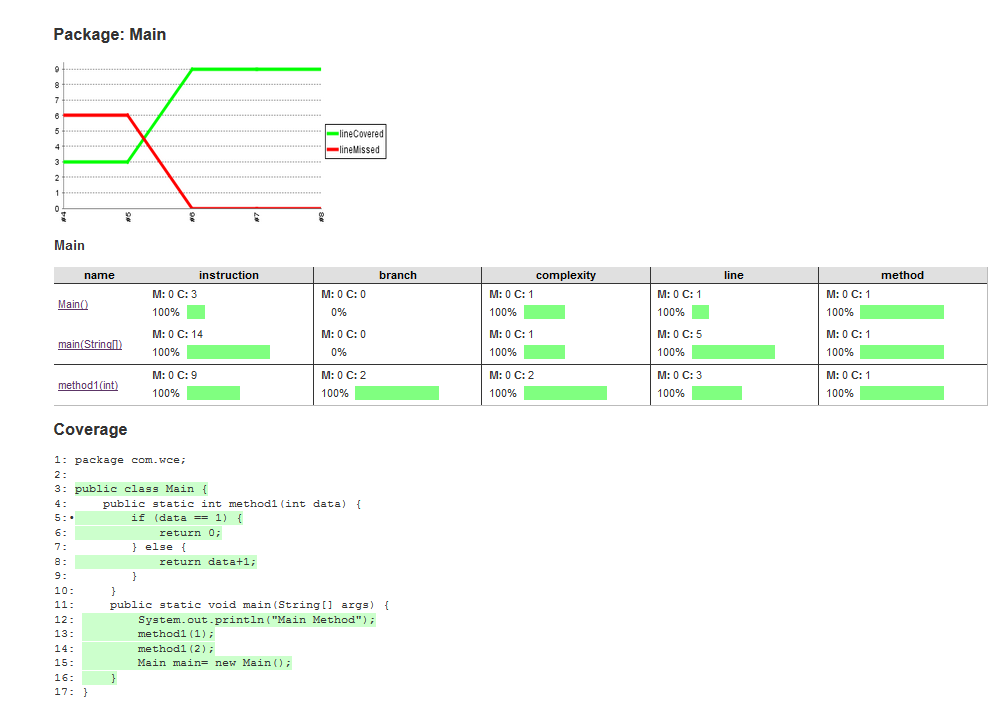
\includegraphics[width=\linewidth]{screenshots/ClassCoverage.png}
			\caption{Class Coverage}
		\end{figure}

	\section{Result}
		Eclipse and Jenkins project is doing code analysis. Jenkins builds daily and publishes report to all teams.
		
				
\chapter{\uppercase{Conclusion and Future Work}}
	\par All teams working on \ac{VRP} are getting coverage analysis regularly. \ac{VRP} is increasing code quality because all developer are writing unit tests to cover all code they have written. 
	\par This project can be extend to find code vulnerabilities in the source code.
\clearpage


\bibliographystyle{IEEETran}
\addcontentsline{toc}{chapter}{Bibliography}
\bibliography{references}

\nocite{*}
\end{document}
